\chapter{Problema de Investigación}


\section{Situación actual} 

Hoy en día el mercado asegurador Venezolano, para poder competir con posee una gran necesidad de adaptarse a las nuevas tecnologías y desarrollar un proceso de 

Actualmente, el proceso de inspección se encuentra realizándose de manera los documentos generados mediante este proceso son físicos por lo cual su persistencia e integridad se ve afectada por el ambiente en donde se resguarden luego de la inspección. Es por ello que con frecuencia se buscan soluciones alternativas que puedan cumplir con el objetivo, de tal manera que se pueda optimizar este proceso, utilizando las tecnologías actuales que estén al alcance de las 

\section{Planteamiento del problema} 
\setlength{\parskip}{5mm}


Actualmente al asistir a la cita para la inspección del vehículo, el perito registra las especificaciones del mismo en una hoja para luego ser archivada y guardada, este proceso se realiza manualmente.

El procesos presenta una serie de inconveniente en cuando a la persistencia de los datos y la administración se refiere:

\begin{itemize}

	\item Las planillas de inspección se guardan solamente en físico.

	\item El riesgo de perder información que no esta respaldada.

	\item El acceso a la información, al ser una búsqueda manual, no es eficiente. 

\end{itemize}


Ante la situación descrita, se plantea elaborar una solución con tecnología Web, que permita a los peritos, mantener un registro digital de las planillas de inspección de los vehículos.

Para ello se propone el desarrollo de la siguiente arquitectura con las siguientes tecnologías:

\newpage
\begin{figure}[H]
\begin{center}
	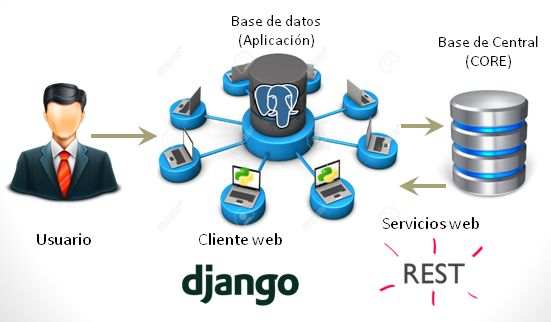
\includegraphics[width=15cm,height=8cm]{img/con_tecnologia1.png}
\end{center}
\caption{Arquitectura Propuesta. Fuente: El Autor.}
\label{fig:Con_Tec_propuesta}
\end{figure}

Para la base de datos utilizaremos PostgreSQL, ya que es una de las bases de datos mas potentes de software libre, con un alto rendimiento, seguridad y a su vez estar disponible prácticamente para todas las versiones de los sistemas operativos Unix y también Windows. Su versatilidad y robustez la hace el candidato perfecto para el sistema que se busca implementar.

Se propone utilizar el framework de Django para el desarrollo del sistema. Ya que siendo uno de los muchos frameworks que están establecidos sobre la base del patrón MVC en sus beneficios se encuentra la separación de responsabilidad y organización del código. Este framework incorpora un patrón llamado MTV (Modelo-Template-Vista), los templates son donde se implementan todas las interfaces de los usuarios, que serán desplegadas por las vistas en el lado del servidor y los mídeles corresponde a la base da datos donde persistirá la información. Además posee un sistema jerárquico de plantilla que proporciona la reutilización de código y la extensibilidad de las aplicaciones. Posee un buen soporte para PostgresSQL, la base de datos que se piensa utilizar para el sistema. 


% Recibirá mediante un web service la información de la planilla y que esta pueda ser editada una vez antes de aceptar y guardarla en el sistema

% Mantener este registro de forma sistematizada 

% Actualmente al asistir a la cita para la inspección del vehiculo, se anotan las especificaciones del mismo en una hoja para luego ser pasada a la computadora, este proceso ocasiona gastos de recursos tanto del personal encargado de traspasar la informacion  como insumos como hojas entre otras  

% Recibirá mediante un web service la información de la planilla y que esta pueda ser editada una vez antes de aceptar y guardarla en el sistema

\setlength{\parskip}{0mm}


% diagrama y arquitectura



\section{Justificación} 
\setlength{\parskip}{5mm}

Un sistema con tecnologías web, es la mejor solución para sistematizar la administración de las planillas de inspección y para el almacenamiento de las mismas de forma digital, para que de esta forma la empresa aseguradora pueda llevar un registro cuyo gestión sea mas eficiente y de múltiple acceso.

La implementación de este sistema representa una reducción riesgos y costos a largo plazo para la compañía, permitiendo que la gestión de las planillas de inspección y los procesos vinculados con ellas se lleven acabo de manera óptima.
\setlength{\parskip}{0mm}

\section{Objetivo general} 

Desarrollar una solución para el proceso de inspección de vehículos en una compañía de seguros.


\section{Objetivos específicos}

\begin{itemize}

	
	
	% \item Permitir la edición de la solicitudes de inspección mediante la aplicación web.
	% \item Análisis y levantamiento de información.

	% \item Diseñar prototipos.

	% \item Diseñar la base de datos.

	% \item Diseñar interfaces de la aplicación web.

	% \item Implementar funcionalidades del sistema.
	% % \item Diseñar e implementar un sistema de registro.

   \item Analizar especificaciones del proceso de inspección de vehículos para suscripción.

   \item Diseñar modelo de datos, de las interfaces y de los componentes de los módulos del sistema.

   \item Desarrollar componentes diseñados.

   \item Realizar pruebas de funcionalidad y de usabilidad.
	
	




	

\end{itemize}





\section{Alcance}

Como alcance del trabajo especial de grado se tiene previsto lograr el registro de usuarios que accederán al sistema para gestionar las planillas, la captura de los datos de la planilla de inspección, la edición de la planilla en caso de incongruencias antes de ser almacenada y guardar el conjunto de datos en la base de datos para su posterior consulta

